%%
% This is an Overleaf template for presentations
% using the TUM Corporate Desing https://www.tum.de/cd
%
% For further details on how to use the template, take a look at our
% GitLab repository and browse through our test documents
% https://gitlab.lrz.de/latex4ei/tum-templates.
%
% The tumbeamer class is based on the beamer class.
% If you need further customization please consult the beamer class guide
% https://ctan.org/pkg/beamer.
% Additional class options are passed down to the base class.
%
% If you encounter any bugs or undesired behaviour, please raise an issue
% in our GitLab repository
% https://gitlab.lrz.de/latex4ei/tum-templates/issues
% and provide a description and minimal working example of your problem.
%%


\documentclass[
  english,            % define the document language (english, german)
  aspectratio=169,    % define the aspect ratio (169, 43)
  % handout=2on1,       % create handout with multiple slides (2on1, 4on1)
  % partpage=false,     % insert page at beginning of parts (true, false)
  % sectionpage=true,   % insert page at beginning of sections (true, false)
]{tumbeamer}


% load additional packages
\usepackage{booktabs}
\usepackage{graphicx}
\usepackage{scrhack} % necessary for listings package
\usepackage{listings}
\lstdefinestyle{mystyle}{
    basicstyle=\ttfamily\footnotesize,
    breakatwhitespace=false,         
    breaklines=true,                 
    captionpos=b,  
    frame=none,
    keepspaces=true,                 
    numbers=none,                    
    numbersep=5pt,
    numberstyle=\small\color{gray},
    showspaces=false,                
    showstringspaces=false,
    showtabs=false,                  
    tabsize=4
}
\lstset{style=mystyle}


% presentation metadata
\title{A Checkpoint Management System for Embedded Distributed Systems}
%\subtitle{Subtitle of the presentation}
\author{Kevin Burton}

\institute{\theChairName\\\theDepartmentName\\\theUniversityName}
\date[01/12/2021]{December 1\textsuperscript{th}, 2021}

\footline{\insertauthor~|~\insertshorttitle~|~\insertshortdate}


% macro to configure the style of the presentation
\TUMbeamersetup{
  title page = TUM tower,         % style of the title page
  part page = TUM toc,            % style of part pages
  section page = TUM toc,         % style of section pages
  content page = TUM more space,  % style of normal content pages
  tower scale = 1.0,              % scaling factor of TUM tower (if used)
  headline = TUM threeliner,      % which variation of headline to use
  footline = TUM default,         % which variation of footline to use
  % configure on which pages headlines and footlines should be printed
  headline on = {title page},
  footline on = {every page, title page=false},
}

% available frame styles for title page, part page, and section page:
% TUM default, TUM tower, TUM centered,
% TUM blue default, TUM blue tower, TUM blue centered,
% TUM shaded default, TUM shaded tower, TUM shaded centered,
% TUM flags
%
% additional frame styles for part page and section page:
% TUM toc
%
% available frame styles for content pages:
% TUM default, TUM more space
%
% available headline options:
% TUM empty, TUM oneliner, TUM twoliner, TUM threeliner, TUM logothreeliner
%
% available footline options:
% TUM empty, TUM default, TUM infoline


\begin{document}

\maketitle

\section{Motivation and Foundations}
\begin{frame}{Motivation}{}
  \begin{figure}
      \centering
      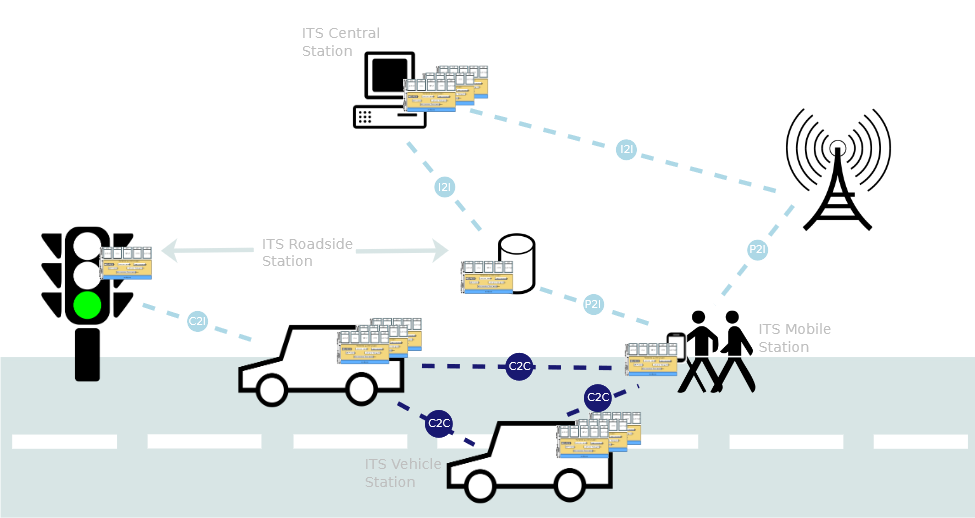
\includegraphics[width=0.75\textwidth]{KIA4SM.PNG}
      \caption{KIA4SM vision - homogeneous platform for heterogeneous devices [1]}
      \label{fig:kia4sm}
  \end{figure}
\end{frame}

\begin{frame}{Foundations}
  \begin{itemize}
      \item Real-Time Checkpoint Restore (RTCR)
  \end{itemize}
\end{frame}

\begin{frame}{Foundations}
  \begin{itemize}
      \item Real-Time Checkpoint Restore (RTCR)
      \item Distributed Shared Memory by Weidinger
  \end{itemize}
\end{frame}

\begin{frame}{Foundations}
\begin{column}{0.3\textwidth}
  \begin{itemize}
      \item RTCR
      \item Weidinger DSM
      \item Genode OS Framework
  \end{itemize}
\end{column}
\begin{column}{0.7\textwidth}\raggedleft
  \begin{figure}
      \centering
      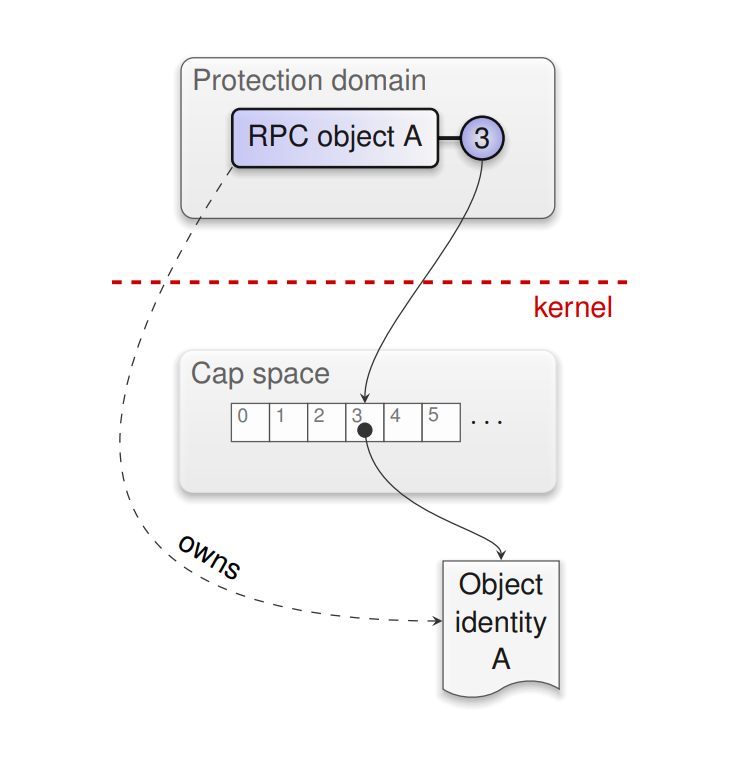
\includegraphics[width=0.45\textwidth]{Cap_space.PNG}
      \caption{Relationship between an RPC object and its corresponding object identity [2, P.41]}
      \label{fig:cap_space}
  \end{figure}
\end{column}
\end{frame}

\section{Concept}
\begin{frame}{Location of the CMS}
\begin{figure}
    \centering
    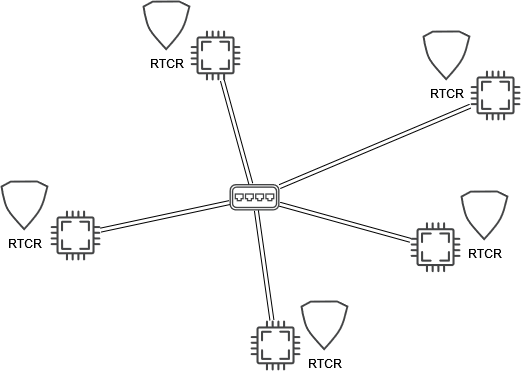
\includegraphics[width=0.5\textwidth]{CMS_Network_topology.png}
    \caption{Network topology}
    \label{fig:network}
\end{figure}
\end{frame}

\begin{frame}{Receiving and Storing of Checkpoints}
\begin{itemize}
    \item Publish/Subscribe
\end{itemize}
\end{frame}

\begin{frame}{Receiving and Storing of Checkpoints}
\begin{itemize}
    \item Publish/Subscribe
    \item Weidinger DSM
\end{itemize}
\end{frame}

\begin{frame}{Receiving and Storing of Checkpoints}
\begin{itemize}
    \item Publish/Subscribe
    \item Weidinger DSM
    \item Hybrid solution
\end{itemize}
\end{frame}

\begin{frame}{Receiving and Storing of Checkpoints}
\begin{figure}
    \centering
    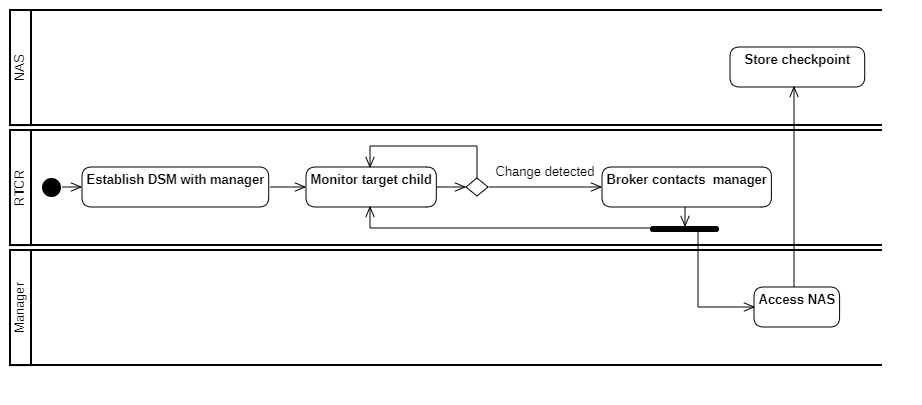
\includegraphics[width=0.75\textwidth]{checkpoint-storing_activity.png}
    \caption{Activity diagram of checkpoint storing}
    \label{fig:storing}
\end{figure}
\end{frame}

\begin{frame}{Migration and Restoration}
\begin{figure}
    \centering
    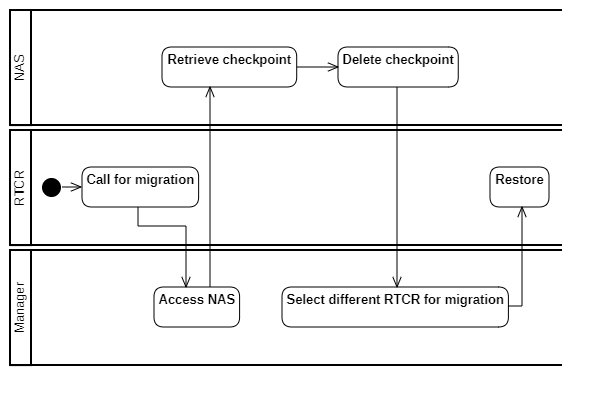
\includegraphics[width=0.5\textwidth]{migration-restoration_activity.png}
    \caption{Activity diagram of migration and restoration}
    \label{fig:migrating}
\end{figure}
\end{frame}

\section{Implementation}
\begin{frame}{Simulating the Infrastructure}
Dummy RTCR
\newline
\begin{itemize}
    \item Establishes DSM
    \item Sends checkpoint
    \item Notifies of checkpoint
    \item Waits for 3 seconds, then calls for migration
\end{itemize}
\end{frame}

\begin{frame}{Simulating the Infrastructure}
DSM
\end{frame}

\begin{frame}{Simulating the Infrastructure}
NIC Router
\begin{figure}
    \centering
    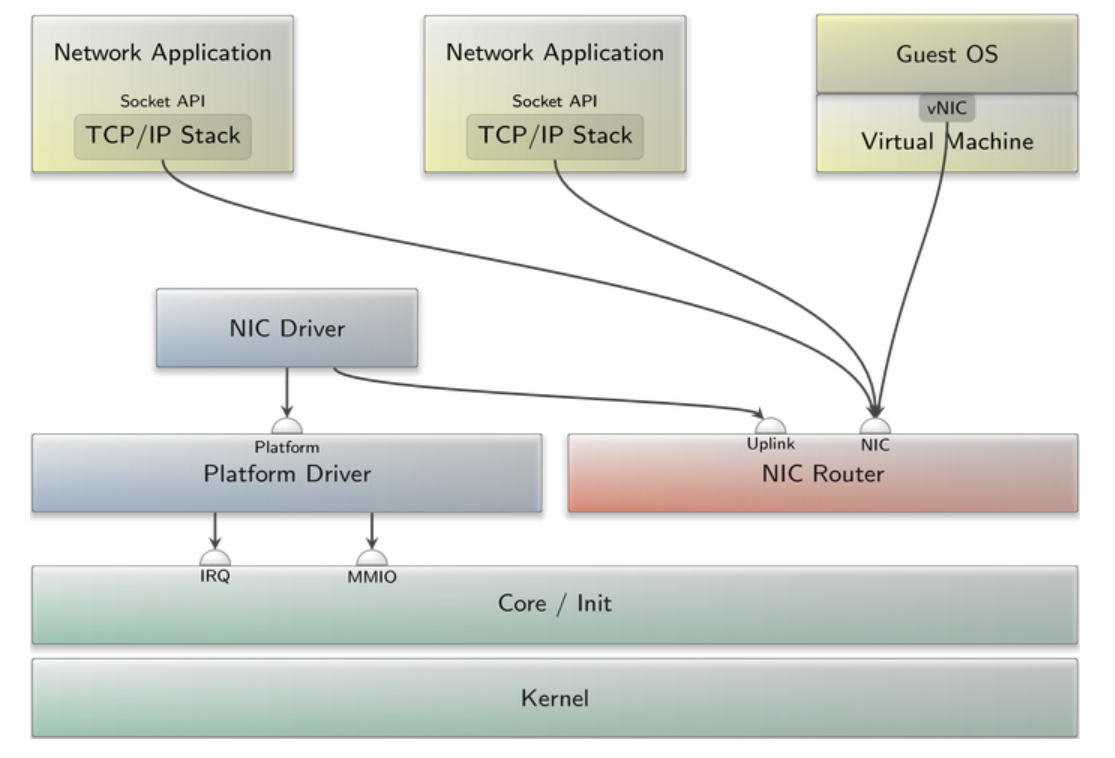
\includegraphics[width=0.5\textwidth]{network_architecture.png}
    \caption{Genode network architecture [3]}
    \label{fig:router}
\end{figure}
\end{frame}

\begin{frame}{Manager}
\hfill
\begin{figure}
    \centering
    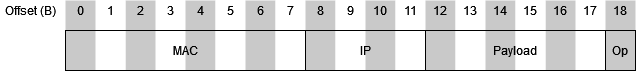
\includegraphics[width=0.7\textwidth]{main_message_format.png}
    \caption{Message format expected on manager interface}
    \label{fig:router}
\end{figure}
\begin{itemize}
    \item Opcode 0: DSM establishment
    \item Opcode 1: Notify of new checkpoint
    \item Opcode 2: Migrate and restore
\end{itemize}
\end{frame}

\begin{frame}{NAS}
\hfill
\begin{figure}
    \centering
    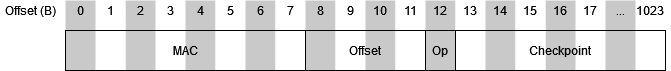
\includegraphics[width=0.7\textwidth]{NAS_message_format_corrected.png}
    \caption{Message format expected on NAS interface}
    \label{fig:router}
\end{figure}
\begin{itemize}
    \item Opcode 0: Store checkpoint
    \item Opcode 1: Retrieve checkpoint
\end{itemize}
\end{frame}

\begin{frame}{}
    \begin{figure}
    \centering
    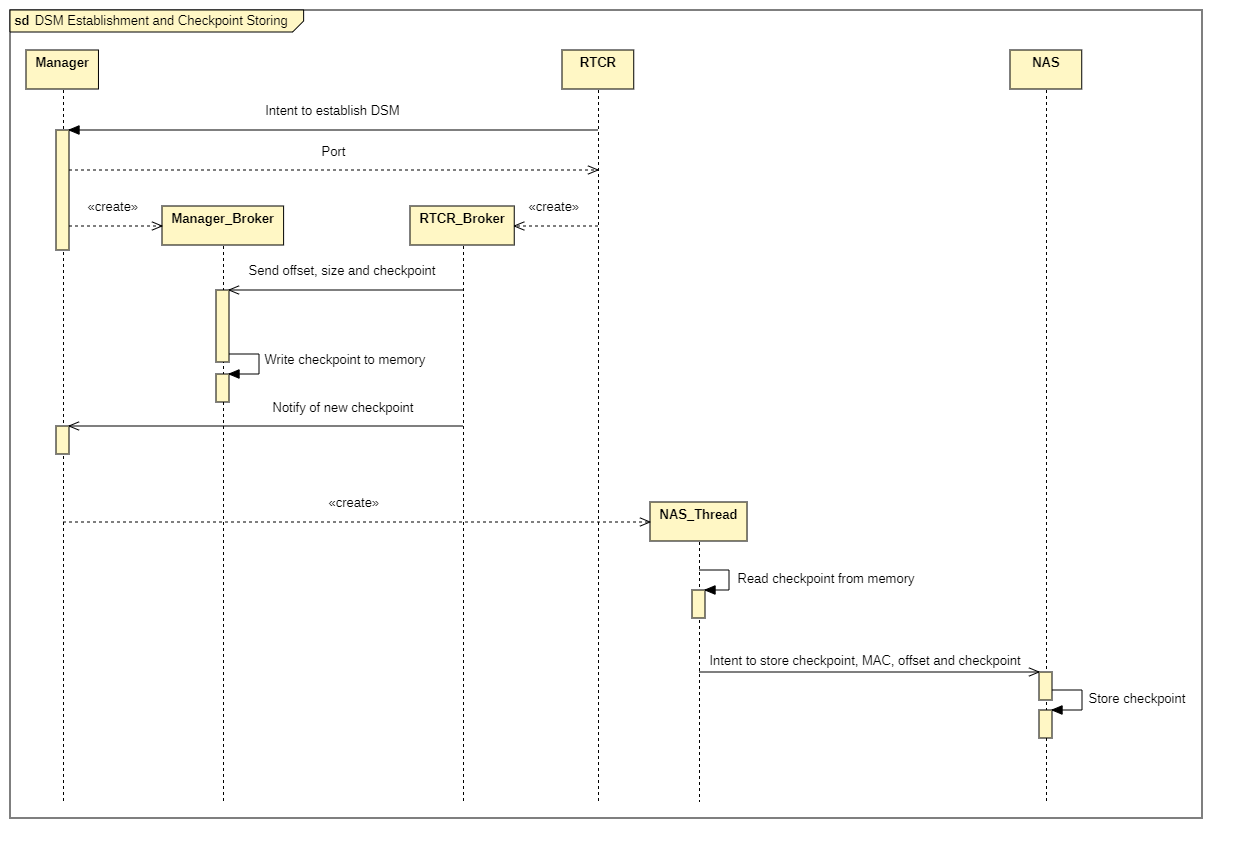
\includegraphics[width=0.8\textwidth]{dsm-and-store_sequence.png}
    \label{fig:router}
\end{figure}
\end{frame}

\section{Evaluation}
\begin{frame}[fragile]{Evaluation}
Output of pseudo-DSM establishment
\begin{lstlisting}
[init -> rtcr_dummy_2] Connecting to manager for DSM establishment
[init -> rtcr_dummy_1] Connecting to manager for DSM establishment
[init -> manager] [broker] Connection to broker successful. Establishing DSM on 1025
[init -> manager] [broker] Done updating memory
[init -> manager] [broker] Connection to broker successful. Establishing DSM on 1026
[init -> manager] [broker] Done updating memory
\end{lstlisting}
\end{frame}

\begin{frame}[fragile]{Evaluation}
Output of checkpoint storing
\begin{lstlisting}
[init -> rtcr_dummy_2] [broker] Notification of new CP sent
[init -> rtcr_dummy_1] [broker] Notification of new CP sent
[init -> manager] [NAS thread] Checkpoint successfully sent to NAS
[init -> nas] Checkpoint was stored successfully
[init -> nas] Checkpoint was stored successfully
[init -> manager] [NAS thread] Checkpoint successfully sent to NAS
\end{lstlisting}
\end{frame}

\begin{frame}[fragile]{Evaluation}
Output of migration and restoration
\begin{lstlisting}
[init -> rtcr_dummy_2] Calling for migration
[init -> rtcr_dummy_1] Calling for migration
[init -> nas] Checkpoint retrieved, sending to manager
[init -> nas] Checkpoint retrieved, sending to manager
[init -> rtcr_dummy_1] [Migr thread] Checkpoint dummy_2 received. Migration successful
[init -> rtcr_dummy_2] [Migr thread] Checkpoint dummy_1 received. Migration successful
\end{lstlisting}
\end{frame}




\section{Limitations and Future Work}
\begin{frame}{Limitations and Future Work}
\begin{enumerate}
    \item Socket connection failure
    \item Redundancy
    \item Distributed shared memory
    \item Dynamic IP and MAC determination
    \item Physical test bench with real hardware NAS
    \item RTCR integration
    \item Real-time capability
\end{enumerate}
\end{frame}

\begin{frame}{Image Sources}
\begin{itemize}
    \item [1] Sebastian Eckl, Daniel Krefft, and Uwe Baumgarten. \textit{KIA4SM - Cooperative Integration Architecture for Future Smart Mobility Solutions.} 2015.
    \item [2] N. Feske. \textit{Genode Operating System Framework 21.05. Foundations [Online].} \url{https://genode.org/documentation/genode-foundations-21-05.pdf}. Accessed on 2021-10-22. 2021.
    \item [3] \textit{Release notes for the Genode OS Framework 21.02. Pluggable network device drivers [Online].} \url{https://genode.org/documentation/release-notes/21.02#Pluggable_network_device_drivers}. Accessed on 2021-10-20.
\end{itemize}
\end{frame}

\end{document}
